\documentclass[vietnamese, 9pt]{article} % beamer neu lam slide

% Nạp các package cần thiết
\usepackage{array}
\usepackage[utf8]{vietnam}
\usepackage[vietnamese]{babel}
\usepackage[top=0.9in, bottom=0.9in, left=0.7in, right=0.7in]{geometry} 
\usepackage{cite} 
\usepackage{hyperref}
\usepackage{titletoc}
\usepackage{graphicx}
\usepackage{color} 
\usepackage{amsmath, amsfonts, amssymb, amsxtra, amsthm}
\usepackage{mathrsfs}
\usepackage{dsfont}
\usepackage{verbatim}
\usepackage[
backend=biber,
style=authortitle,
sorting=none
]{biblatex}
\addbibresource{references.bib}


% Định nghĩa lệnh mới






% Định nghĩa môi trường mới
\theoremstyle{definition}
\newtheorem{dn}{Định nghĩa}[section]
\newtheorem{dly}[dn]{Định lý}
\newtheorem{md}[dn]{Mệnh đề}
\newtheorem{hq}[dn]{Hệ quả}
\newtheorem{bd}[dn]{Bổ đề}
\newtheorem{vd}[dn]{Ví dụ}
\newtheorem{gt}[dn]{Giả thuyết}
\newtheorem{bt}{Bài tập}[section]
\newtheorem{rmk}{Chú ý}
\newtheorem{nota}{Quy ước}
\newtheorem{fact}{Tính chất}
\newtheorem{nx}{Nhận xét}
\newtheorem{ly}{Lưu ý}
\theoremstyle{remark}
\renewcommand\thesection{\Roman{section}}
\renewcommand\thesubsection{\arabic{subsection}}
\renewcommand\theparagraph{\thesubsubsubsection.\arabic{paragraph}}
%\newtheorem{bt}{Bài tập}[section]
%\newtheorem*{rmk}{Chú ý}
%\newtheorem*{nota}{Quy ước}
%\newtheorem*{fact}{Tính chất}
\usepackage{titlesec}
\usepackage{hyperref}

\titleclass{\subsubsubsection}{straight}[\subsection]

\newcounter{subsubsubsection}[subsubsection]
\renewcommand\thesubsubsubsection{\thesubsubsection.\arabic{subsubsubsection}}
\renewcommand\theparagraph{\thesubsubsubsection.\arabic{paragraph}} % optional; useful if paragraphs are to be numbered

\titleformat{\subsubsubsection}
  {\normalfont\normalsize\bfseries}{\thesubsubsubsection}{1em}{}
\titlespacing*{\subsubsubsection}
{0pt}{3.25ex plus 1ex minus .2ex}{1.5ex plus .2ex}

\makeatletter
\renewcommand\paragraph{\@startsection{paragraph}{5}{\z@}%
  {3.25ex \@plus1ex \@minus.2ex}%
  {-1em}%
  {\normalfont\normalsize\bfseries}}
\renewcommand\subparagraph{\@startsection{subparagraph}{6}{\parindent}%
  {3.25ex \@plus1ex \@minus .2ex}%
  {-1em}%
  {\normalfont\normalsize\bfseries}}
\def\toclevel@subsubsubsection{4}
\def\toclevel@paragraph{5}
\def\toclevel@paragraph{6}
\def\l@subsubsubsection{\@dottedtocline{4}{7em}{4em}}
\def\l@paragraph{\@dottedtocline{5}{10em}{5em}}
\def\l@subparagraph{\@dottedtocline{6}{14em}{6em}}
\makeatother

\setcounter{secnumdepth}{4}
\setcounter{tocdepth}{4}

\numberwithin{equation}{section}
\setcounter{MaxMatrixCols}{15}


\begin{document}




\newpage
\tableofcontents % mục lục


\newpage
\section{Tóm tắt ý tưởng giải quyết vấn đề}
Vấn đề cần giải quyết: đại dịch covid-19 xuất hiện không chỉ đe dọa sức khỏe thể chất mà còn gây ra những ảnh hưởng tiêu cực đến sức khỏe tinh thần của con người. Vì vậy mỗi con người cần phải cải thiện và tối ưu hóa chất lượng cuộc sống.
\subsection{Những yếu tố cần xét đến}
\begin{itemize}
    \item Những yếu tố (domain) và khía cạnh (facet) ảnh hưởng tới chất lượng cuộc sống.
    \item Mối quan hệ giữa các domain và facet.
\end{itemize}
\subsection{Ý tưởng giải quyết vấn đề}
\begin{itemize}
    \item Lập bảng để chỉ ra những domain và các facet tương ứng ảnh hưởng tới chất lượng cuộc sống.
    \item Với mỗi domain, xây dựng cách để đánh giá chất lượng, sự ảnh hưởng của domain đó tới cuộc sống. Trong bài báo cáo này, thang đo cho sự đánh giá sẽ là $100$.
    \item Vì độ ảnh hưởng của mỗi domain tới cuộc sống là khác nhau nên ta sẽ làm khảo sát để đánh giá độ ảnh hưởng của mỗi domain đến chất lượng cuộc sống (lấy theo thang $5$). Độ ảnh hưởng của mỗi domain sẽ là trung bình cộng của các đánh giá về độ ảnh hưởng của domain đó làm tròn đến $2$ chữ số thập phân.
    \item Xây dựng công thức tính chất lượng cuộc sống: ta nhân chất lượng mỗi domain với độ ảnh hưởng tương ứng của nó, cộng lại với nhau rồi chia cho tổng các độ ảnh hưởng.\\
    Ví dụ: chất lượng và độ ảnh hưởng của domain $A_1, A_2,..., A_n$ lần lượt là $x_1, x_2,..., x_n$ và $y_1, y_2,..., y_n$. Khi đó chất lượng cuộc sống, đặt là $X$, được tính bằng công thức:
    $$X = \frac{x_1y_1 + x_2y_2 + ... + x_ny_n}{y_1 + y_2 + ... + y_n}$$
    \item Dựa theo bảng khảo sát, chọn ra $3$ domain có độ ảnh hưởng lớn nhất và cải thiện nó.
    \item Lên plan cho mùa dịch.
\end{itemize}
\begin{ly}
Các số liệu về tài chính mang tính giả định cao, các công thức không chính xác hoàn toàn. Mục đích của bài báo cáo là để đưa ra đánh giá và các giải pháp tốt nhất có thể.
\end{ly}
\section{Những Domain và Facet ảnh hưởng đến chất lượng cuộc sống}
Sự hài lòng về chất lượng cuộc sống là mức độ cảm nhận hay cảm xúc của con người về những điều mà con người có được trong cuộc sống. Những điều đó bao gồm cả những yếu tố về vật chất lẫn tinh thần. Hài lòng với chất lượng cuộc sống thì con người mới cảm thấy hạnh phúc và thoải mái. Dựa vào các tiêu chí của công ty Mercer, nhóm mình đã rút ra được các domain chính và các facet tương ứng để đánh giá chất lượng cuộc sống, được thể hiện ở bảng dưới [1].
\begin{center}
\begin{tabular}{ | m{1.1cm} | m{4cm}| m{6.5cm} | } 
  \hline
  STT& Domain & Facet \\ 
  \hline
  1 & Văn hóa xã hội & - Cách cư xử, ý thức xã hội. \newline - Các mối quan hệ gia đình và xã hội. \newline - Nam nữ bình đẳng. \newline - Khu dân cư có nhiều tiện ích đáp ứng được nhu cầu rèn luyện sức khỏe.\\ 
  \hline
  2 & An ninh quốc phòng & - Môi trường sống an toàn. \newline - Xã hội trật tự, kỉ cương. \newline - Sống yên bình trên cơ sở các quy phạm pháp luật và chuẩn mực đạo đức, pháp lý xác định sẵn.  \\ 
  \hline
  3 & Môi trường tự nhiên & - Đất đai, nước, không khí, động thực vật, thời tiết,... \\ 
  \hline
  4 & Giáo dục và đào tạo & Chất lượng của trường học phổ thông, cao đẳng và đại  học. \newline - Chương trình đào tạo. \newline - Phương pháp giảng dạy. \newline - Cơ sở vật chất. \\ 
  \hline
  5 & Cơ sở hạ tầng & - Hệ thống điện. \newline - Hệ thống cấp - thoát nước. \newline - Giao thông thuận lợi, bố trí hợp lý. \newline - Dịch vụ viễn thông (điện thoại, internet). \newline - Dịch vụ bưu chính. \newline - Các cơ sở giáo dục, y tế, văn hoá. \\ 
  \hline
  6 & Thu nhập & - Môi trường làm việc, cơ hội nâng cao thu nhập. \newline - Chính sách hỗ trợ, vay vốn. \newline - Dịch vụ ngân hàng.\\ 
  \hline
  7 & Y tế và chăm sóc sức khỏe & - Chế độ lương thực, dinh dưỡng. \newline - Chế độ luyện tập. \newline - Chế độ nghỉ ngơi, giải trí. \\ 
  \hline
\end{tabular}
\end{center}
\section{Công thức đánh giá chất lượng cuộc sống}
\subsection{Xây dựng công thức đánh giá chất lượng từng domain}
\subsubsection{Đánh giá theo thanh ngang}
\textbf{Giới thiệu về phương pháp:} ta sẽ dùng phương pháp cảm quan để đánh giá chất lượng của một số domain. Phương pháp này là phương pháp đánh giá chất lượng dựa trên việc sử dụng các thông tin thu được qua sự cảm nhận của các cơ quan con người khi tiếp xúc, đối mặt với các vấn đề như: thị giác, thính giác, khứu giác, xúc giác và vị giác. Các cơ quan có vai trò thu nhận các cảm giác về các chỉ tiêu chất lượng và đưa ra điểm số.\\
Để dễ hình dung hơn, nhóm mình sẽ gọi đây là phương pháp đánh giá theo thanh ngang. Chất lượng của mỗi facet được đưa ra sẽ được đánh giá theo mức điểm từ $1$ đến $100$, dựa theo bảng sau:
\begin{center}
\begin{tabular}{| m{2cm}| m{3cm} | m{2.8cm} | m{2.8cm} | m{2.8cm} | m{2.8cm}|} 
  \hline
  Cảm nhận & Rất không hài lòng & Không hài lòng &Bình thường & Hài lòng& Rất hài lòng\\ 
  \hline
  Mức điểm& $1-20$ & $21-40$ & $41-60$ & $61-80$ & $81-100$ \\ 
  \hline
\end{tabular}
\end{center}
Ta sẽ đánh giá chất lượng từng facet của mỗi domain bằng điểm số từ $1$ đến $100$. Chất lượng của domain đó sẽ là trung bình cộng chất lượng các facet được đưa ra.\\
Ưu điểm:
\begin{itemize}
    \item Hầu như không tốn chi phí.
    \item Là một trong những phương pháp đơn giản nhất.
\end{itemize}
Nhược điểm:
\begin{itemize}
    \item Mức độ chính xác không quá cao.
    \item Độ chính xác của dự đoán phụ thuộc lớn vào trình độ, kinh nghiệm, thói quen của người dự đoán.
\end{itemize}
Phương pháp đánh giá bằng thanh ngang sẽ dùng để đánh giá các domain: văn hóa xã hội, giáo dục và đào tạo, cơ sở hạ tầng. Tiếp đến nhóm mình sẽ liệt kê các facet tương ứng với mỗi domain phục vụ cho phương pháp đánh giá bằng thanh ngang này.
\subsubsection{Văn hóa xã hội}
Câu hỏi đặt ra cho chúng ta là làm sao đánh giá, đo lường được văn hóa xã hội khi nó có đặc tính vô hình, nó là một khái niệm khá trừu tượng, vốn dĩ là cái không “sờ mó” được? Dưới đây là một số yếu tố được sử dụng phổ biến nhất hiện nay để đánh giá, đo lường tác động của văn hóa đối với đời sống con người:
\subsubsubsection{Những quá trình và cấu trúc hữu hình}
Là những giá trị có thể dễ nhìn thấy, nghe thấy, cảm nhận được bao gồm:
\begin{itemize}
    \item Các thành tựu, sản phẩm truyền thống lâu đời.
    \item Lễ nghi và lễ hội hàng năm.
    \item Các biểu tượng, hình ảnh đặc trưng.
    \item Ngôn ngữ, trang phục, các trò chơi dân gian, truyền thống.
    \item Những câu chuyện, giai thoại, sử thi.
\end{itemize}
\subsubsubsection{Những giá trị được chia sẻ, được chấp nhận, được tuyên truyền}
Là những giá trị trải qua quá trình hoạt động lâu dài, được người dân, nhà nước chấp nhận, phổ biến và áp dụng bao gồm:
\begin{itemize}
    \item Những chuẩn mực hành vi. 
    \item Tập quán, tập tục.
    \item Nghi thức, tín ngưỡng.
\end{itemize}
\subsubsubsection{Những quan niệm chung}
Là những giá trị hình thành sau một thời gian hoạt  động, ghi dấu ấn vào tâm lý hầu hết các người dân và gần như không thể thay đổi, làm khác đi, trở thành điều mặc nhiên được công nhận. Chúng định hướng cho suy nghĩ, cảm nhận và hành vi của các thành viên trong cả mối quan hệ bên trong và bên ngoài gia đình và xã hội bao gồm:
\begin{itemize}
    \item Các giá trị đời sống tinh thần. 
    \item Các quan niệm, tư tưởng.
    \item Các quan niệm để phát triển.
    \item Hệ tư tưởng.
\end{itemize}
Với mỗi khía cạnh nhỏ của từng khía cạnh, ta sẽ đánh giá chất lượng của nó theo phương pháp thanh ngang. Chất lượng của từng khía cạnh sẽ là trung bình cộng chất lượng các khía cạnh nhỏ tương ứng (ví dụ như khía cạnh những giá trị được chấp nhận, được tuyên truyền gồm có những khía cạnh nhỏ là những chuẩn mực, hành vi, tập quán, tập tục và nghi thức, tín ngưỡng). Từ đó xây dựng công thức tính chất lượng của văn hóa xã hội bằng cách lấy trung bình cộng của chất lượng các khía cạnh.
\subsubsection{Giáo dục và đào tạo}
\subsubsubsection{Chương trình và chất lượng đào tạo}
\begin{itemize}
    \item Giáo viên có trình độ tốt, được tạo điều kiện để phát triển.
    \item Chương trình dạy đánh giá đúng quá trình và kết quả giáo dục.
\end{itemize}
\subsubsubsection{Phương pháp giảng dạy}
\begin{itemize}
    \item Cập nhật các phương pháp giảng dạy mới, luôn thay đổi để theo kịp với thời đại.
    \item Phương pháp giảng dạy thích hợp với người dạy và người học.
\end{itemize}
\subsubsubsection{Cơ sở vật chất}
\begin{itemize}
    \item Thiết bị công nghệ, học liệu giáo dục dễ tiếp cận.
    \item Trang bị đầy đủ các trang thiết bị phục vụ cho việc dạy học.
    \item Các trang thiết bị phải đảm bảo chất lượng tốt.
\end{itemize}
Với mỗi khía cạnh nhỏ của từng khía cạnh, ta sẽ đánh giá chất lượng của nó theo phương pháp thanh ngang. Chất lượng của từng khía cạnh sẽ là trung bình cộng chất lượng các khía cạnh nhỏ tương ứng. Từ đó xây dựng công thức tính chất lượng của giáo dục và đào tạo bằng cách lấy trung bình cộng của chất lượng các khía cạnh.
\subsubsection{Cơ sở hạ tầng}
Ta xét đến các khía cạnh của dịch vụ công, cơ sở hạ tầng
\subsubsubsection{Hệ thống điện}
\begin{itemize}
    \item Điện được cung cấp đầy đủ, ổn định, giá cả hợp lý.
\end{itemize}
\subsubsubsection{Hệ thống cấp - thoát nước}
\begin{itemize}
    \item Nước sạch được cung cấp đầy đủ, ổn định.
    \item Tiêu thoát nước dễ dàng, không gây ô nhiễm môi trường
\end{itemize}
\subsubsubsection{Hệ thống giao thông vận tải}
\begin{itemize}
    \item Đường giao thông thuận lợi, dễ dàng.
    \item Phương tiện giao thông công cộng bố trí hợp lý, thuận lợi.
    \item Không gây ô nhiễm môi trường.
\end{itemize}
\subsubsubsection{Dịch vụ viễn thông}
\begin{itemize}
    \item Dịch vụ viễn thông (điện thoại, internet) được cung cấp tốt, giá cả hợp lý.
\end{itemize}
\subsubsubsection{Dịch vụ truyền hình}
\begin{itemize}
    \item Dịch vụ truyền hình (Cable,tivi,..) được cung cấp tốt, giá cả hợp lý.
\end{itemize}
\subsubsubsection{Dịch vụ bưu chính}
\begin{itemize}
    \item Bưu kiện được gửi - nhận đầy đủ, an toàn, an ninh (bảo mật), nhanh chóng, giá cả hợp lý.
\end{itemize}
\subsubsubsection{Cơ sở giáo dục, y tế, văn hoá xã hội}
\begin{itemize}
    \item Trường học, bệnh viện và các công trình công cộng được bố trí hợp lý, thuận lợi.
\end{itemize}
Với mỗi khía cạnh nhỏ của từng khía cạnh, ta sẽ đánh giá chất lượng của nó theo phương pháp thanh ngang. Chất lượng của từng khía cạnh sẽ là trung bình cộng chất lượng các khía cạnh nhỏ tương ứng. Từ đó xây dựng công thức tính chất lượng của cơ sở hạ tầng bằng cách lấy trung bình cộng của chất lượng các khía cạnh.
\subsubsection{Môi trường tự nhiên}
Xét các yếu tố để xây dựng công thức đánh giá môi trường tự nhiên:\\
Chất lượng tiếng ồn hằng ngày: $A$\\
Gọi $B$(dB) là giá trị trung bình của tiếng ồn [11] trong 1 ngày.
\begin{itemize}
\item $B \leq 80$ là mức độ con người có thể nghe được mà không cần thiết bị bảo vệ nên $A \geq 90$\\
Từ đó ta có: $A=100-\frac{B}{8}$
\item $80 < B \leq 90$ có hại cho thính giác nếu tiếp xúc trong thời gian dài (từ 1 tiếng trở lên) nên $90 > A \geq 10$\\
Từ đó ta có: $A=100-(8B-630)$
\item $90 < B \leq 100$ rất có hại cho thính giác nếu tiếp xúc trong thời gian dài (từ 15 phút đến 1 tiếng) nên $A<10$\\
Từ đó ta có: $A=100-B$
\item $100 \leq B$ cực kì có hại, không chịu được quá 15 phút nên $A = 0$
\end{itemize}
Chất lượng bầu không khí: $C$\\
Gọi $D$ là chỉ số chất lượng không khí AQI [10] ở Việt Nam
\begin{itemize}
\item Nếu $D \leq 150$ thì $C=100-\frac{2}{3}D$
\item Nếu $D > 150$ thì $C=0$
\end{itemize}
Mức độ ảnh hưởng của thiên tai tới khu vực đang sống: $E$, được đánh giá trên thang điểm từ $0$ đến $100$.
\begin{center}
        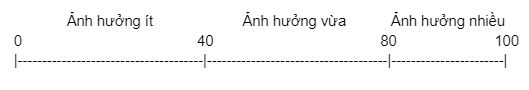
\includegraphics[scale=0.6]{2.png}
\end{center}
Từ đó ta xây dựng được công thức tính chất lượng môi trường tự nhiên là:
$$\frac{1}{3}[A + C + (100 - E)]$$
\subsubsection{An ninh quốc phòng}
Xét các yếu tố để xây dựng công thức đánh giá chất lượng an toàn, an ninh:\\
An ninh trật tự ở địa phương
\begin{itemize}
    \item Tỉ lệ trộm cắp, xảy ra mâu thuẫn ở địa phương: $A$\\
    \begin{center}
        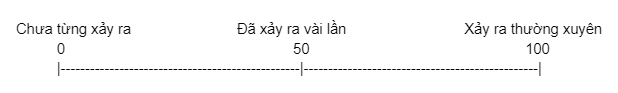
\includegraphics[scale=0.6]{1.png}
    \end{center}
    \item Tỉ lệ tệ nạn xã hội(rượu chè, cờ bạc, ma túy,..) ở địa phương: $B$\\
    \begin{center}
        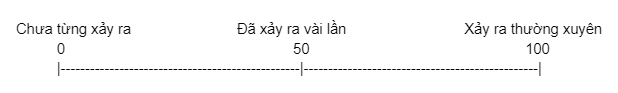
\includegraphics[scale=0.6]{1.png}
    \end{center}
\end{itemize}
An toàn giao thông
\begin{itemize}
    \item (Tỉ lệ số đèn giao thông/số nơi có giao cắt giữa các tuyến đường)x$100$: $C$
    \item Tỉ lệ biển báo giao thông ở những chỗ nguy hiểm (ngã 3, ngã 4, giao nhau với đường ưu tiên,...): $D (\%)$
    \item Tỉ lệ người không tuân thủ an toàn giao thông (vượt đèn giao thông, không đội mũ bảo hiểm, phóng nhanh, vượt ẩu,...): $E$\\
    \begin{center}
        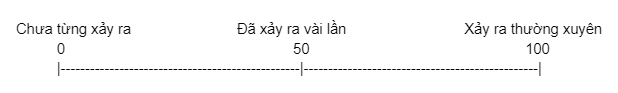
\includegraphics[scale=0.6]{1.png}
    \end{center}
\end{itemize}
Từ đó ta xây dựng được công thức tính chất lượng an toàn, an ninh chung ở địa phương:
$$\frac{1}{4}[(100 - A) + (100 - B) + C + D + (100 - E)]$$
\subsubsection{Thu nhập}
Các khoản chi tiêu trong mùa dịch [2] sẽ được chia làm hai phần chính
\subsubsubsection{Nhu cầu vật chất}
\begin{itemize}
\item Đi lại: chi phí dùng cho việc di chuyển. Vì đang trong mùa dịch nên thường mọi người sẽ hạn chế đi ra ngoài, chỉ đi bằng xe riêng của mình để đi làm hoặc mua những đồ dùng yếu phẩm. 100k/tháng (tiền xăng, bảo dưỡng, sửa xe,...).
\item Bảo vệ sức khỏe: các khoản như khám chữa bệnh, tiền thuốc, bảo hiểm y tế,... 200k/tháng.
\item Ăn, mặc, ở: quần áo, tiền ăn, tiền điện, nước,... 4000k/tháng.
\end{itemize}
\subsubsubsection{Nhu cầu văn hóa tinh thần}
\begin{itemize}
\item Học tập: học thêm, sách vở, đồ dùng học tập…. 1000k/tháng.
\item Nghỉ ngơi, giải trí: đi chơi, đi xem phim,... 500k/tháng.
\item Giao tiếp xã hội: đám tiệc, hội họp, thăm viếng,.... Vì dịch bệnh nên khoản này có thể bỏ qua.
\item Ngoài ra, phải dành một số tiền tiết kiệm, dự phòng,... chiếm $50 \%$ trong tổng số tiền chi tiêu hàng tháng.
\end{itemize}
Vậy ta có khoản chi tiêu tổng cộng trong 1 tháng là: (100k + 200k + 4000k + 1000k + 500k)/$50 \%$ = 11600k.\\
Nếu thu nhập mỗi tháng lớn hơn hoặc bằng 11600k thì chất lượng thu nhập là 100.\\
Nếu ngược lại thì chất lượng thu nhập sẽ được tính bằng công thức: (Tổng số tiền thu nhập/tổng số tiền phải chi tiêu hàng tháng)x100 = (Tổng số tiền thu nhập/11600k)x100.
\begin{nota}
$1k$ = $1000$ VND
\end{nota}
\subsubsection{Y tế và chăm sóc sức khỏe}
Để đảm bảo có sức khỏe tốt, ta cần để ý đến các yếu tố
\subsubsubsection{Chất lượng, dinh dưỡng bữa ăn và chế độ luyện tập}
Giả sử một người nam (nữ) giới trưởng thành có chiều cao, cân nặng trung bình muốn duy trì sức khoẻ hiện tại (chiều cao, cân nặng).\\ Ta có công thức tính tỷ lệ trao đổi chất cơ bản (Basal Metabolic Rate - BMR) [3]:\\
Đặt $a$ là khối lượng cơ thể theo kg, $b$ là chiều cao cơ thể theo cm, $c$ là số tuổi. Công thức được phát biểu như sau:
\begin{itemize}
\item Đối với nam giới:
$$BMR = 66,5+(13,75.a)+(5,003.b)-(6,755.c)$$
\item Đối với nữ giới: 
$$BMR=55,1+(9,563.a)+(1,850.b)-(4,676.c)$$
\end{itemize}
Chỉ số này cho ta biết mức năng lượng tối thiểu mà cơ thể cần để đảm bảo duy trì các hoạt động bình thường.
Từ đó ta có tổng lượng calories tiêu thụ/ngày: $TDEE = BMR.R$
\begin{center}
\begin{tabular}{| m{2cm}|m{2.8cm}| m{2.8cm} | m{2.8cm} | m{2.8cm} | m{2.8cm}|} 
  \hline
  Đối tượng& Ít vận động& Vận động nhẹ\newline (1-3 lần/tuần) &Vận động vừa \newline (3-5 lần/tuần) & Vận động nặng \newline (6-7 lần/tuần)& Vận động rất nặng \newline (2 lần/ngày)\\ 
  \hline
  R& $1,2$ & $1,375$ & $1,55$ & $1,725$ & $1,9$ \\ 
  \hline
\end{tabular}
\end{center}
Đặt $t = |A - TDEE|$ là lượng calo thừa hoặc thiếu đối với việc duy trì cơ thể.\\
Công thức chất lượng dinh dưỡng: $$X = (1 -\frac{t}{TDEE}).100$$
Trong đó $A$ là lượng calo nạp vào cơ thể. Chất lượng bằng $0$ nếu $t \geq TDEE$.\\
Phạm vi tin cậy [4] $95 \%$ đối với nam giới là ± $213.0$ kcal/ngày và ± $201.0$ kcal/ngày đối với phụ nữ.
\subsubsubsection{Nguồn thuốc thiết yếu}
Được đánh giá theo phương pháp thanh ngang với 2 tiêu chí
\begin{itemize}
\item Nguồn thuốc được duy trì đầy đủ, an toàn. Đặt là $Y_1$.
    \begin{center}
        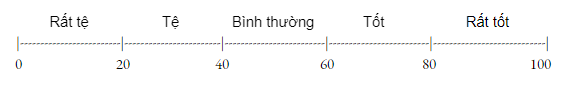
\includegraphics[scale=0.6]{3.png}
    \end{center}
\item Giá cả hợp lý. Đặt là $Y_2$
    \begin{center}
        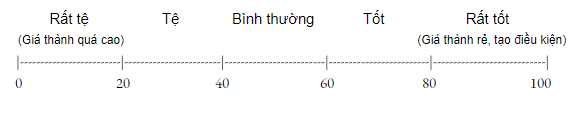
\includegraphics[scale=0.6]{4.png}
    \end{center}
\end{itemize}
Công thức đánh giá chất lượng nguồn thuốc:
$$Y = \frac{Y_1 + Y_2}{2}$$
\subsubsubsection{Vệ sinh và thu gom rác thải}
Đặt chất lượng vệ sinh và thu gom rác thải là là $Z$, ta sẽ đánh giá theo phương pháp thanh ngang với mức điểm số như sau
\begin{center}
        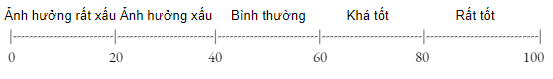
\includegraphics[scale=0.6]{5.png}
\end{center}
\subsubsubsection{Tình hình dịch bệnh ở địa phương}
Đặt chất lượng tình hình dịch bệnh ở địa phương là $T$, ta sẽ đánh giá theo phương pháp thanh ngang với mức điểm số như sau
\begin{center}
        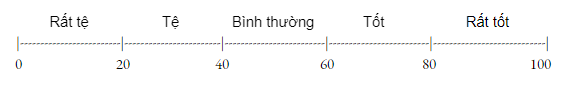
\includegraphics[scale=0.6]{3.png}
\end{center}
Ta xây dựng được công thức đánh giá chất lượng sức khỏe là
$$\frac{X + Y + Z + T}{4}$$
\subsection{Công thức đánh giá chất lượng cuộc sống}
Khi khảo sát độ quan trọng của từng domain trong bảng ở phần II, chúng mình đã thu được kết quả như sau:
\begin{center}
   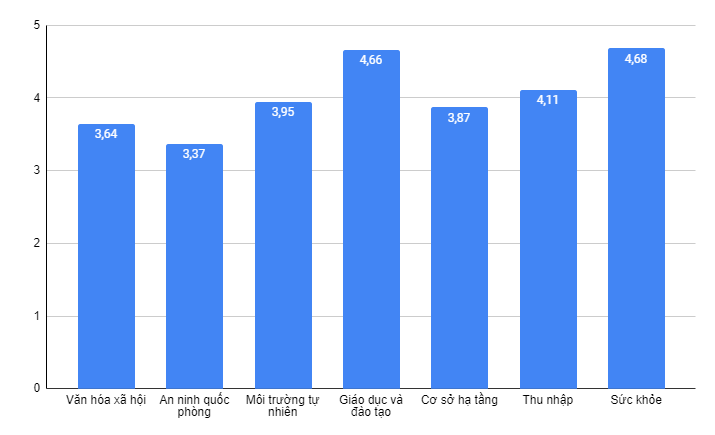
\includegraphics[scale=0.6]{6.png} 
\end{center}
Trong biểu đồ này, độ quan trọng tương ứng của từng domain là trung bình cộng của các đánh giá về độ quan trọng của domain đó, làm tròn đến $2$ chữ số thập phân.\\
Gọi chất lượng của các domain ứng với mỗi cá nhân trong biểu đồ từ trái qua phải lần lượt là $x_1, x_2,..., x_7$ với $x_i \in \mathbb{N}$, $0 \leq x_i \leq 100$. Khi đó ta xây dựng được công thức tính chất lượng cuộc sống, đặt là $X$, là:
$$X = \frac{x_1.3,64 + x_2.3,37 + x_3.3,95 + x_4.4,66 + x_5.3,87 + x_6.4,11 + x_7.4,68}{3,64 + 3,37+ 3,95+ 4,66+ 3,87 + 4,11 +4,68}$$
Công thức trên được viết lại gọn hơn là:
$$X = \frac{x_1.3,64 + x_2.3,37 + x_3.3,95 + x_4.4,66 + x_5.3,87 + x_6.4,11 + x_7.4,68}{28,28}$$
\textbf{Bảng khảo sát:} <https://bom.to/zR4QzLhqDreeVr>
\section{Nâng cao chất lượng cuộc sống và xây dựng plan}
Trong biểu đồ đánh giá độ quan trọng của từng domain ở phần III, ta chọn ra được $3$ domain ảnh hưởng nhất đến chất lượng cuộc sống là: giáo dục và đào tạo, sức khỏe, thu nhập. Tiếp đến, nhóm mình sẽ bàn về việc nâng cao chất lượng và xây dựng plan để tối ưu hóa cuộc sống.
\subsection{Y tế và chăm sóc sức khỏe}
Để có một sức khỏe tốt, dinh dưỡng là một điều không thể thiếu. Tìm hiểu về chế độ ăn uống và đưa ra thực đơn hợp lý là một cách tốt để đảm bảo về sức khỏe và sự phát triển của bản thân. Do đó, nhóm mình sẽ lập nên một thực đơn ăn uống trong vòng một tuần để có hiệu quả tốt nhất.\\
Chúng ta sẽ xây dựng mô hình về thực đơn ăn uống dựa trên giá trị dinh dưỡng của suất ăn hay tính toán về lượng calo cho một suất ăn bất kì.\\
Giả sử cần phải lập thực đơn ăn uống trong một tuần cho một bạn nam có chiều cao 1m75, nặng 70kg và đang ở độ tuổi 18.\\
Áp dụng công thức tính tỉ lệ trao đổi chất cơ bản, ta có mức năng lượng cơ thể cần để đảm bảo duy trì các hoạt động bình thường là:
$$BMR = 66,5 + 13,75.70 + 5,003.175 - 6,755.18 = 1782,935$$
Giả sử mức vận động của người đó ở mức vừa (3 - 5 lần/tuần), khi đó tổng lượng kcal tiêu thụ/ngày là:
$$TDEE = BMR.R = 1782,935.1,55 = 2763,54925$$
Do đó, để duy trì được năng lượng cơ thể thì mỗi ngày phải cung cấp xấp xỉ 2763,54925 kcal.\\
Chúng ta đều biết rằng kcal là thứ quan trọng mà chúng ta nói tới một món ăn hay suất ăn cụ thể. Do đó ta sẽ lập các bảng thống kê về giá trị dinh dưỡng của các món ăn tính theo đơn vị kcal. Các món ăn sẽ được chia làm các phần: món sáng, món mặn, món rau, món canh, món súp và ăn vặt [5].
\begin{center}
\begin{tabular}{ | m{1cm} | m{4cm}| m{3cm} | m{4cm}|}
 \hline
 \multicolumn{4}{|c|}{Món sáng} \\
 \hline
  STT& Tên món & Số lượng & Giá trị năng lượng (kcal) \\ 
\hline
  1 & Xôi xéo & 200 gram & 334 \\ 
 \hline
  2 & Bánh mì thịt & 1 ổ & 318 \\ 
 \hline
   3& Phở bò & 1 tô & 315 \\ 
 \hline
   4 & Mì tôm & 1 tô & 129 \\ 
 \hline
   5 & Cháo sườn & 1 tô & 255 \\ 
 \hline
   6 & Bún riêu cua & 1 tô & 362 \\ 
 \hline
   7 & Bánh bao nhân thịt & 1 chiếc & 211 \\ 
 \hline
\end{tabular}
\end{center}


\begin{center}
\begin{tabular}{ | m{1cm} | m{4cm}| m{3cm} | m{4cm}|}
 \hline
 \multicolumn{4}{|c|}{Món mặn} \\
 \hline
  STT& Tên món & Số lượng & Giá trị năng lượng (kcal) \\ 
\hline
  1 & Salad ức gà & 1 dĩa & 225 \\ 
 \hline
  2 & Thịt gà xào rau củ & 1 dĩa & 301 \\ 
 \hline
   3& Thịt bò kho tiêu & 1 dĩa & 333 \\ 
 \hline
   4 & Thịt bò hầm khoai tây & 1 tô & 516 \\ 
 \hline
   5 & Cá sốt cà chua & 1 dĩa & 415 \\ 
 \hline
   6 & Cá rán & 1 dĩa & 432 \\ 
 \hline
   7 & Thịt heo kho trứng & 1 dĩa & 339 \\ 
 \hline
    8 & Thịt heo luộc & 1 dĩa & 270 \\ 
 \hline
    9 & Tôm kho & 1 dĩa & 287 \\ 
 \hline
    10 & Tôm nấu măng & 1 tô & 268 \\ 
 \hline
    11 & Mực nhồi thịt hấp & 1 dĩa & 301 \\ 
 \hline
    12 & Mực chiên xù & 1 dĩa & 312 \\ 
 \hline
    13 & Xúc xích & 100 gram & 315 \\ 
 \hline
    14 & Chả lụa & 2 chiếc & 134 \\ 
 \hline
\end{tabular}
\end{center}



\begin{center}
\begin{tabular}{ | m{1cm} | m{4cm}| m{3cm} | m{4cm}|}
 \hline
 \multicolumn{4}{|c|}{Món rau} \\
 \hline
  STT& Tên món & Số lượng & Giá trị năng lượng (kcal) \\ 
\hline
  1 & Rau muống luộc & 1 dĩa & 115 \\ 
 \hline
  2 & Rau muống xào & 1 dĩa & 168\\ 
 \hline
   3& Rau cải luộc & 1 dĩa & 121 \\ 
 \hline
   4 & Rau cải xào & 1 dĩa & 165 \\ 
 \hline
   5 & Rau dền luộc & 1 dĩa & 177 \\ 
 \hline
   6 & Mướp xào & 1 dĩa & 239 \\ 
 \hline
   7 & Salad dưa chuột cà chua & 1 dĩa & 197 \\ 
 \hline
    8 & Giá xào & 1 dĩa & 168 \\ 
 \hline
    9 & Nấm xào & 1 dĩa & 202 \\ 
 \hline
    10 & Ngọn bí xào tỏi & 1 dĩa & 162 \\ 
 \hline
\end{tabular}
\end{center}



\begin{center}
\begin{tabular}{ | m{1cm} | m{4cm}| m{3cm} | m{4cm}|}
 \hline
 \multicolumn{4}{|c|}{Món canh, súp} \\
 \hline
  STT& Tên món & Số lượng & Giá trị năng lượng (kcal) \\ 
\hline
  1 & Canh rau ngót & 1 tô & 155 \\ 
 \hline
  2 & Canh bầu nấu tôm & 1 tô & 327\\ 
 \hline
   3& Canh su hào & 1 tô & 245 \\ 
 \hline
   4 & Canh mồng tơi nấu cua & 1 tô & 226 \\ 
 \hline
   5 & Canh rau cải & 1 tô & 216 \\ 
 \hline
   6 & Canh chua & 1 tô & 366 \\ 
 \hline
   7 & Súp nấm & 1 tô & 215 \\ 
 \hline
    8 & Súp bí đỏ & 1 tô & 404 \\ 
 \hline
    9 & Súp rong biển & 1 tô & 299 \\ 
 \hline
    10 & Súp ngô hải sản & 1 tô & 316 \\ 
 \hline
\end{tabular}
\end{center}



\begin{center}
\begin{tabular}{ | m{1cm} | m{4cm}| m{3cm} | m{4cm}|}
 \hline
 \multicolumn{4}{|c|}{Ăn vặt} \\
 \hline
  STT& Tên món & Số lượng & Giá trị năng lượng (kcal) \\ 
\hline
  1 & Bơ & 100 gram & 160 \\ 
 \hline
  2 & Táo & 100 gram & 52 \\ 
 \hline
   3& Cam & 100 gram & 47 \\ 
 \hline
   4 & Nhãn & 100 gram & 62 \\ 
 \hline
   5 & Xoài & 100 gram & 60 \\ 
 \hline
   6 & Dâu tây & 100 gram & 32 \\ 
 \hline
   7 & Na & 100 gram & 101 \\ 
 \hline
    8 & Mít sấy & 50 gram & 131 \\ 
 \hline
    9 & Hạt hướng dương & 50 gram & 292 \\ 
 \hline
    10 & Hạt điều & 50 gram & 286 \\ 
 \hline
    11 & Bánh quy hạnh nhân & 50 gram & 166 \\ 
 \hline
    12 & Bánh quy phô mai & 50 gram & 221 \\ 
 \hline
    13 & Chè khúc bạch & 1 ly & 264 \\ 
 \hline
    14 & Chè đậu đen & 1 ly & 278 \\ 
 \hline
\end{tabular}
\end{center}
Tiếp theo ta sẽ sắp xếp các món ăn trên vào thực đơn 1 tuần gồm 7 ngày, sao cho:
\begin{itemize}
    \item Mỗi ngày gồm : bữa sáng, bữa trưa, bữa tối và bữa phụ.
    \item Bữa sáng gồm 1 món ăn sáng.
    \item Bữa trưa và bữa tối mỗi bữa gồm cơm, 2 món mặn (khác nhau), 1 món rau và 1 món canh hoặc súp.
    \item Bữa phụ gồm 2 món ăn vặt (trong đó có 1 món trái cây).
    \item Đặt $T_i$ với $i \in \mathbb{N}, 1 \leq i \leq 7$ là tổng lượng kcal ngày thứ $i$ từ thực đơn và $X_i= |T_i - 2763,54925|$. Ta sẽ xây dựng thực đơn sao cho các giá trị $X_i$ không quá lớn.
\end{itemize}
Để tối ưu hoá thực đơn và hạn chế số lần thực hiện ta xây dựng thực đơn cơ bản bằng cách:
\begin{itemize}
    \item Cho các món ăn sáng có kcal tăng dần từ ngày 1 đến ngày 7.
    \item Bữa trưa kcal món mặn 1 tăng dần, món mặn 2 giảm dần, món rau tăng dần, món canh giảm dần (theo thứ tự ngày $1, 2, 3, 4, 5, 6, 7$).
    \item Bữa tối kcal món mặn 1 tăng dần, món rau giảm dần (theo thứ tự ngày 2,3,4,5,6,7,1), kcal món mặn 2 giảm dần, món canh tăng dần (theo thứ tự ngày 4,5,6,7,1,2,3).
    \item Bữa phụ có kcal trái cây tăng dần và kcal ăn vặt giảm dần.
\end{itemize}
Ta xây dựng được thực đơn cho 7 ngày trong 1 tuần như sau:
\begin{center}
\begin{tabular}{ | m{0.8cm} | m{2cm}| m{3cm} |m{3cm} | m{3.2cm} | m{2.2cm} |m{1cm} |}
 \hline
  Ngày & Bữa sáng & Bữa trưa & Bữa tối & Bữa phụ & Tổng kcal ($T_i$) & $X_i$\\ 
\hline
  1 & Mì tôm & Chả lụa \newline Thịt bò hầm khoai tây \newline Rau muống luộc\newline Súp bí đỏ& Thịt gà xào rau củ \newline Thịt bò kho tiêu \newline Rau cải xào \newline Canh mồng tơi nấu cua & Dâu tây \newline Hạt hướng dương & 2781 & 17,45 \\ 
 \hline
  2 & Bánh bao & Salad ức gà \newline Cá rán \newline Rau cải luộc \newline Canh chua & Chả lụa \newline Xúc xích \newline Mướp xào \newline Súp rong biển & Cam \newline Hạt điều & 2813 & 49,45 \\ 
 \hline
  3 & Cháo sườn & Tôm nấu măng \newline Cá sốt cà chua \newline Ngọn bí xào tỏi \newline Canh bầu nấu tôm & Salad ức gà \newline Mực chiên xù \newline Nấm xào \newline Súp ngô hải sản & Táo \newline Chè đậu đen & 2946 & 182,45 \\ 
 \hline
  4 & Phở bò  & Thịt heo luộc \newline Thịt bò kho tiêu \newline Rau cải xào \newline Súp ngô hải sản & Tôm nấu măng \newline Thịt bò hầm khoai tây \newline Salad dưa chuột cà chua \newline Canh rau ngót  & Xoài \newline Chè khúc bạch & 2993 & 229,45 \\ 
 \hline
  5 & Bánh mì thịt & Tôm kho \newline Thịt kho trứng \newline Giá xào \newline Súp rong biển & Thịt heo luộc \newline Cá rán \newline Rau dền luộc \newline Súp nấm & Nhãn \newline Bánh quy vị phô mai & 2922 & 158,45 \\ 
 \hline
  6 & Xôi xéo & Mực nhồi thịt hấp \newline Xúc xích \newline Rau muống xào \newline Canh su hào  &Tôm kho \newline Cá sốt cà chua \newline Giá xào \newline Canh rau cải  & Na \newline  Bánh quy hạnh nhân & 2850 & 86,45 \\ 
 \hline
  7 & Bún riêu cua  & Thịt gà xào rau củ \newline Mực chiên xù \newline Rau dền luộc \newline Canh mồng tơi nấu cua & Mực nhồi thịt hấp \newline Thịt heo kho trứng \newline Rau muống xào \newline Canh su hào & Bơ \newline Mít sấy & 2856 & 92,45 \\ 
 \hline
\end{tabular}
\end{center}
\begin{ly}
Khi tính tổng kcal $(T_i)$, ngoài các món ăn kể trên còn bao gồm 134 kcal từ cơm mỗi ngày.
\end{ly}
\subsection{Giáo dục và đào tạo}
\textbf{Tình hình thực tế:} trước tình hình dịch Covid-19 diễn biến phức tạp thì việc học tập tại các cơ sở dưới hình thức tập trung trực tiếp gần như bị gián đoạn hoàn toàn.\\ 
Để có thể giải quyết vấn đề 1 cách đơn giản hơn ta đặt ra một vài số liệu có tính tương đối như sau:
\begin{itemize}
    \item $100 \%$ việc học tập trong mùa dịch được thực hiện tại nhà hoặc trực tuyến.
    \item Giấc ngủ trung bình của người Việt Nam [6] vào khoảng 7h/ngày.
    \item Khoảng thời gian trung bình người Việt  dùng cho các hoạt động khác:
    \begin{itemize}
        \item Ăn uống: 1,5h/ngày (30’/ bữa).
        \item Tập thể dục thể thao: 0,5h/ngày.
        \item Giải trí (chủ yếu thuộc về sử dụng Smartphone) [7]: 5,1h/ngày.
        \item Sinh hoạt trong gia đình: 2,21h/ngày (2,89h/ngày đối với nữ và 1,53h/ngày đối với nam).
    \end{itemize}
\end{itemize}
Kết luận: Khoảng thời gian trung bình còn lại dùng cho vấn đề giáo dục vào khoảng 7,69h/ngày (Lưu ý khoảng thời gian này chỉ là tương đối và sẽ có sai số tuỳ thuộc vào thói quen sinh hoạt từng người).\\

Tiếp theo, ta sẽ tìm hiểu về các khung giờ học tập để mang lại hiệu quả tốt nhất
\begin{itemize}
    \item 4h30 - 6h: học lý thuyết\\
     Theo nghiên cứu, đây là khung giờ lý tưởng để bắt đầu học thuộc lòng, bởi giờ này không khí yên tĩnh, đầu óc sáng suốt do đó não dễ tiếp nhận thông tin hơn.
    \item 7h15 - 10h: Khung giờ cho các môn xã hội, văn học, ngôn ngữ \\
    Đây là khoảng thời gian rất tốt để học các môn liên quan đến xã hội, ngôn ngữ, văn học. Các môn này đòi hỏi việc ghi nhớ các kiến thức liên quan đến sáng tạo và ít đòi hỏi tư duy logic.
    \item 14h - 16h30: khung giờ tốt nhất cho các môn tự nhiên\\
    Buổi chiều là khoảng thời gian vô cùng thích hợp để học các môn tự nhiên đòi hỏi tư duy logic và tính toán nhiều. Một số cách để giảm bớt căng thẳng trong khoảng thời gian này đó chính là nghe những bài nhạc không lời và có khoảng nghỉ giữa chừng trong thời gian học.
    \item 19h45 - 22h30: thời gian dành cho các môn tính toán, logic\\
    Vào khoảng thời gian cuối ngày, não bộ sẽ không còn được sung sức dành cho các môn học thuộc lòng nữa,  không nên học các kiến thức quá khó vì sẽ khiến chúng ta nhanh chán, mệt mỏi. Cách tốt nhất là tận dụng khung giờ này để học các môn tính toán, có thể áp dụng công thức. Do đó, nên tận dụng khung giờ này để làm bài tập các môn tự nhiên như Toán, Lý, Hóa.
\end{itemize}
Lưu ý cho việc học tập được tốt hơn:  Để giảm bớt căng thẳng trong quãng thời gian học tập thì chúng ta có thể nghe những bài nhạc không lời. Ngoài ra, sau 45 phút - 1 giờ học tập nên rời bàn học và nghỉ ngơi từ 5 đến 10 phút. Quãng thời gian nghỉ ngơi này giúp chúng ta lấy lại năng lượng để việc học được tiếp tục một cách hiệu quả hơn. Đặc biệt, tránh vào mạng xã hội vì sẽ khiến bị phân tâm và cám dỗ.
\textbf{Chuẩn bị trước khi lập plan}
\begin{itemize}
    \item Đánh giá năng lực hiện tại của bản thân
    \begin{itemize}
        \item Vừa mới tham dự xong kì thi THPTQG. Các kiến thức để học khi lên ĐH (đại cương toán, lí,...) vẫn chưa có.
        \item Làm bài kiểm tra năng lực tiếng anh đạt mức tương đương 5.0 IELTS.
        \item Xuất thân là chuyên Toán nên các kiến thức về lập trình chưa được tiếp xúc nhiều, trong khi bản thân sẽ theo học về IT.
        \item Khá yếu các môn về xã hội và muốn tìm hiểu thêm về nó.
    \end{itemize}
    \item Mục tiêu học tập
    \begin{itemize}
        \item Nâng band IELTS lên 6.0 trong 2 tháng hè, học tiếng anh hàng ngày.
        \item Học trước về các môn đại cương trong chương trình ĐH, có đủ năng lực để tham dự cuộc thi cấp trường diễn ra vào khoảng tháng 3 năm sau.
        \item Tìm hiểu về lập trình, ôn luyện để tham gia thi cấp trường bảng không chuyên vào tháng 11.
        \item Đọc thêm sách, truyện.
        \item Việc học tập không quá nặng vì vừa kết thúc 12 năm đèn sách vất vả.
    \end{itemize}
\end{itemize}
\subsection{Thu nhập}
\textbf{Tình hình thực tế:}
Tính đến tháng 12 năm 2020, cả nước có 32,1 triệu người từ 15 tuổi trở lên bị ảnh hưởng tiêu cực bởi dịch Covid-19 bao gồm người bị mất việc làm, phải nghỉ giãn việc/nghỉ luân phiên, giảm giờ làm, giảm thu nhập,… Trong đó, $69,2 \%$ người bị giảm thu nhập, $39,9 \%$ phải giảm giờ làm/nghỉ giãn việc/nghỉ luân phiên và khoảng $14,0 \%$ buộc phải tạm nghỉ hoặc tạm ngừng hoạt động sản xuất kinh doanh. [8]\\
Trung bình chi tiêu hàng tháng của một người trong mùa dịch sẽ gồm các khoản
\begin{itemize}
    \item Khoản tiêu dùng ngắn hạn: là các khoản chi tiêu cần thiết chiếm phần lớn trong tổng chi tiêu hàng tháng bao gồm
    \begin{itemize}
        \item Chi tiêu cá nhân ( ăn uống, mua sắm, tiền điện thoại, trả nợ cả nhân, khác).
        \item Chi tiêu nhà cửa ( tiền thuê nhà, tiền mua nhà, tiền điện, tiền nước, truyền hình, phí dịch vụ nhà).
        \item Chi tiêu đi lại (tiền xăng, tiền đi lại khác).
        \item Chi tiêu gia đình (tiền học phí cho con cái/ tiền tiêu vặt cho con nếu có gia đình).
    \end{itemize}
    \item Khoản tiêu dùng dài hạn: đây là các khoản tích góp để dành từng tháng để mua/ chi cho những khoản lớn (cưới hỏi, mua xe, nhà cửa, du lịch).
    \item Khoản dành cho phát triển cá nhân: đây là khoản trống để đầu tư cho mình về kiến thức bằng các khóa học hoặc tài liệu sách vở là chính là đầu tư cho tương lai.
\end{itemize}
Tiếp đến ta sẽ bàn về các khoản thu nhập trong thời gian dịch bệnh.\\
Những số liệu dưới đây chỉ mang tính tương đối vì có thể mức lương sẽ khác nhau tùy thuộc vào chất lượng công việc (cùng một công việc nhưng làm ra thành phẩm có yêu cầu độ khó, độ tinh vi cao hơn sẽ được nhiều tiền hơn) hoặc phụ thuộc vào nơi làm việc (như việc dạy thêm ở thành phố sẽ có mức lương cao hơn ở những vùng nông thôn) nên tôi chỉ đưa ra số liệu có tính tương đối và khái quát cao nhất (theo kinh nghiệm cá nhân và các trang thông tin việc làm trên internet) để tiện cho việc lập plan sau này.
\begin{itemize}
    \item Đối với những cá nhân ở khu vực không bị ảnh hưởng bởi dịch Covid-19: những công việc chính vẫn sẽ được duy trì nên sẽ thu được mức thu nhập ổn định, cụ thể theo số liệu thống kê, vào năm 2020, thu nhập bình quân tháng đạt 5,5 triệu đồng [9].
    \item Đối với những cá nhân ở khu vực bị ảnh hưởng bợi dịch Covid-19 hoặc những cá nhân chưa có việc làm chính (như sinh viên, người mới ra trường,...): có thể làm những công việc làm thêm tại nhà (work from home) để kiếm thu nhập hàng tháng.
\end{itemize}
Có thể tìm việc làm thêm ở các trang web lớn trên mạng như: vietnamworks, jobstreet, timviecnhanh,.... hoặc các group tìm việc trên facebook như: Job opportunities - Internship, HR - INTERNSHIP & CAREER OPPORTUNITIES.\\
Những việc phổ biến có thể làm thêm tại nhà trong thời gian dịch bệnh:\\
\textbf{Việc làm đồ thủ công:} người làm sẽ nhận làm thêm các công việc gia công tại nhà (như thêu tranh, làm đồ handmade,...). Thu nhập dao động trung bình từ 500.000 VNĐ cho đến 2.000.000 VNĐ (hoặc có thể hơn) một tháng.\\
\textbf{Việc làm trực tuyến qua các phương tiện hiện đại:} để có thể làm việc từ xa hiệu quả cần có sự chuẩn bị như việc đảm bảo máy tính có kết nối internet ổn định, sử dụng thành thạo các phần mềm riêng của doanh nghiệp,.. Ta có thể kể đến một số công việc như sau:
\begin{itemize}
    \item Làm cộng tác viên viết bài: người làm sẽ nhận yêu cầu và viết bài chuẩn SEO về đa dạng lĩnh vực (như bóng đá, thời trang, đồ ăn,...) từ các công ty hoặc trên những trang web trên internet. Thu nhập dao động từ 5.000.000 VNĐ cho đến 10.000.000 VNĐ (hoặc có thể hơn) một tháng.
    \item Dịch thuật tại nhà: người làm nếu có năng khiếu về ngoại ngữ có thể nhận dịch văn bản hoặc phim. Thu nhập trung bình khi dịch một văn bản là 35.000 VND đến 200.000 VNĐ và một bộ phim là 150.000 VNĐ đến 200.000 VNĐ.
    \item Gia sư online tại nhà: công việc dành cho những người có kiến thức và khả năng truyền đạt tốt. Đây là công việc sẽ không tốn nhiều thời gian mà đem lại nguồn thu nhập ổn định. Người làm sẽ nhận dạy thêm (cho một trung tâm tiếng anh hoặc trung tâm dạy toán,....). Thu nhập trung bình của việc dạy cho một trung tâm tiếng anh sẽ là khoảng 50.000 VNĐ đến 60.000 VNĐ/1 giờ, thu nhập 1 tháng sẽ dao động từ 2.000.000 VNĐ đến 5.000.000 VNĐ.
    \item chăm fanpage/Trực page Facebook: người làm sẽ quản lý page facebook, công việc chỉ đòi hỏi người làm có thời gian 4-5 tiếng/1 ngày , không bắt buộc cố định và lương cũng nằm ở mức ổn. Thu nhập mỗi giờ dao động khoản từ 20.000 VNĐ đến 30.000 VNĐ, mỗi tháng khoảng từ 2.400.000 VNĐ đến 4.500.000 VNĐ.
    \item Designer online: hiện nay, công việc này đang được rất nhiều cá nhân và nhà tuyển dụng ưa chuộng. Các công ty hướng đến thuê design freelance để giải quyết công việc nhanh chóng và tiết kiệm được chi phí. Người làm chỉ cần dành khoảng 4-5h mỗi ngày. Thu nhập dao động từ 2.500.000 VNĐ đến 5.000.000 VNĐ một tháng.
\end{itemize}

Từ đó ta lập được bảng về plan trong giáo dục đào tạo và thu nhập trong 2 tháng hè như sau
\begin{center}
\begin{tabular}{ | m{2.5cm} | m{7.5cm}| m{7.5cm} |}
 \hline
 \multicolumn{3}{|c|}{4 tuần đầu} \\
 \hline
  Nội dung & Lịch trình & Ghi chú \\ 
\hline
 Tiếng anh & Dành ra 2-3 giờ/ngày (buổi sáng) \newline Listening: \newline - Rèn luyện phần phát âm để tránh nhầm lẫn khi nghe. \newline - Tích luỹ từ vựng và trau dồi ngữ pháp về các chủ đề thường gặp trong Listening. \newline Reading: \newline - Tự phân loại và học từ vựng theo các chủ đề. \newline Speaking: \newline - Đầu tư vào phần phát âm. \newline Writing: \newline - Trau dồi vốn từ vựng của một sô chủ đề phổ biến trong IELTS Writing: cách dùng từ, cách diễn đạt. \newline - Nắm chắc cách dùng và cấu trúc ngữ pháp cần thiết. \newline Kết hợp học trên những trang mạng xã hội như facebook, có thể học nhóm với bạn bè: nói chuyện bằng tiếng anh. \newline Làm bài test ôn lại kiến thức sau 4 tuần học& - Đây là khoảng thời gian mới bắt đầu nên cần tập trung vào những nội dung cơ bản như từ vựng, phát âm, ngữ pháp và tạo cho bản thân chiến lược làm bài hiệu quả. \newline - Đối với phần Speaking và Writing có thể gửi bài cho thầy cô chấm và chữa thường xuyên. \newline - Tránh việc học trong một khoảng thời gian quá dài dẫn đến chán nản thì có thể giải lao giữa giờ, có thể kết hợp khoảng thời gian này để nghe nhạc bằng tiếng anh. \\ 
 \hline
 Lập trình & Dành ra 1-2 giờ/ngày (buổi chiều hoặc tối) \newline - Tìm kiếm các khóa học online để làm quen với lập trình. Một số khóa học cơ bản như: C++ for beginners của Codelearn hoặc Codecademy. \newline - Tìm hiểu thêm về thiết kế website qua khóa Responsive Web Design của freecodecamp. & - Đây là khoảng thời gian để làm quen với lập trình và lựa chọn ngôn ngữ lập trình bắt đầu. \\ 
 \hline
 Đại cương các môn: toán, lý& Dành ra 1-2 giờ/ngày (buổi chiều hoặc tối) \newline - Tìm hiểu về đại cương các môn toán, lý ở chương trình đại học qua mạng. Sau đó sẽ tìm một tài liệu phù hợp với bản thân để theo học. Nó có thể là giáo trình của các trường ĐH trong nước, ngoài nước hoặc các cuốn sách chuyên sâu. \newline - Học và làm quen với các kiến thức cơ bản của đại cương theo các tài liệu đã tìm kiếm được ở trên. & - Nên nhờ các anh chị đi trước tư vấn để có được lộ trình học đúng nhất, không bị lệch hướng. \\ 
 \hline
 Kiến thức xã hội và giải trí & Dành ra 45 phút-1 giờ/ ngày (buổi tối) \newline - Đọc một số sách vừa có tính giải trí, vừa có tính nâng cao kiến thức. & - Đọc các cuốn truyện kinh điển như Harry Potter, Sherlock Holmes hoặc những truyện tranh ngắn viết bằng tiếng anh. \newlinw - Xem các bộ phim ngắn tập hoặc dài tập tùy thích. \\
 \hline
Thu nhập & Dạy thêm qua Zoom cho học sinh chuẩn bị lên lớp 12 ôn thi đại học (Toán, Lý, Hóa) & - Mỗi tuần dạy 2 buổi (thời gian dạy có thể linh hoạt tùy thuộc vào người học) mỗi buổi kéo dài 3 tiếng từ 8h-11h đêm. Lương một buổi 300.000 VNĐ. Thu nhập một tháng khoảng 3.900.000 VNĐ \\ 
 \hline
\end{tabular}
\end{center}





\begin{center}
\begin{tabular}{ | m{2.5cm} | m{7.5cm}| m{7.5cm} |}
 \hline
 \multicolumn{3}{|c|}{4 tuần sau} \\
 \hline
  Nội dung & Lịch trình & Ghi chú \\ 
\hline
 Tiếng anh & Dành ra 2-3 giờ/ngày (buổi sáng) \newline Listening: \newline - Luyện tập các kỹ năng nâng cao như scanning, skimming, note-taking để không bỏ lỡ ý. \newline - Kiểm tra và phân tích đáp án sau khi làm bài. \newline Reading: \newline - Luyện tập và giải đề thường xuyên với độ khó tăng dần. \newline Speaking: \newline  - Luyện tập phát âm thường xuyên để tăng phản xạ và nói trôi chảy. \newline Writing: \newline - Luyện tập thường xuyên. \newline Tham khảo bài mẫu và thường xuyên gửi cho thầy cô chấm và sửa. \newline Thường xuyên đọc báo, tin tức, xem phim, nghe nhạc bằng tiếng anh. \newline Làm bài test ôn lại kiến thức sau 8 tuần học. & - Đây là khoảng thời gian tăng thời lượng học và tăng tốc giải các dạng đề để đạt kết quả.\\ 
 \hline
 Lập trình & Dành ra 1-2 giờ/ngày (buổi chiều hoặc tối) \newline - Khi đã quen với các kiến thức cơ bản, ta sẽ bắt đầu học những khóa học cao hơn như: C++ advanced, Data Science. \newline - Luyện kỹ năng về thuật toán ở những trang như codeforces, VNOI. \newline - Tìm hiểu về các dạng đề và làm thử đề thi olympic tin học cấp trường các năm trước nhằm chuẩn bị cho cuộc thi được diễn ra vào tháng 11. & - Trong giai đoạn này, khi đã bắt đầu quen với kiến thức cơ bản, ta sẽ tiếp xúc với những kiến thức sâu và rộng hơn. \\ 
 \hline
 Đại cương các môn: toán, lý& Dành ra 1-2 giờ/ngày (buổi chiều hoặc tối) \newline - Tiếp tục học để hoàn thiện những kiến thức căn bản của đại cương. Ngoài ra, có thể tham gia vào các diễn đàn để thảo luận nhằm nâng cao hơn kiến thức của bản thân. & - Hoàn thiện và nắm chắc kiến thức. \\ 
 \hline
 Kiến thức xã hội và giải trí & Dành ra 45 phút-1 giờ/ ngày (buổi tối) \newline - Đọc một số sách vừa có tính giải trí, vừa có tính nâng cao kiến thức tránh gây chán & - Đọc các cuốn truyện kinh điển như Harry Potter, Sherlock Holmes hoặc những truyện tranh ngắn viết bằng tiếng anh. \newlinw - Xem các bộ phim ngắn tập hoặc dài tập tùy thích. \\
 \hline
Thu nhập 1 & Dạy thêm qua Zoom cho học sinh chuẩn bị lên lớp 12 ôn thi đại học (Toán, Lý, Hóa) & - Mỗi tuần dạy 2 buổi (thời gian dạy có thể linh hoạt tùy thuộc vào người học) mỗi buổi kéo dài 3 tiếng từ 8h-11h đêm. Lương một buổi 300.000 VNĐ. Thu nhập một tháng khoảng 3.900.000 VNĐ \\ 
 \hline
 Thu nhập 2 & - Dịch thuật tại nhà: nhận dịch văn bản hoặc phim. \newline - Làm cộng tác viên viết bài (bóng đá, thời trang, đồ ăn,...) từ các công ty, web. & - Có thể thực hiện bất cứ lúc nào có thời gian rảnh còn lại. Thu nhập trung bình khi dịch một văn bản là 35.000 VND đến 200.000 VNĐ và một bộ phim là 150.000 VNĐ đến 200.000 VNĐ.\\
 \hline
\end{tabular}
\end{center}
\section{Đánh giá về mô hình}
\subsection{Ưu điểm}
\begin{itemize}
    \item Các mô hình không quá phức tạp, dễ tính toán.
    \item Các công thức xây dựng trong bài có thể không mang lại kết quả đúng nhất nhưng đơn giản và dễ làm. Trên thực tế, đối với việc mô hình hóa bài toán, thay vì mất nhiều thời gian để xử lý bài toán một cách chính xác gần như tuyệt đối thì việc sử dụng các thuật toán đơn giản hơn dù không ra được kết quả tốt nhất vẫn được sử dụng phổ biến.
    \item Có tính thực tiễn.
    \item Đối với sức khỏe
    \begin{itemize}
        \item Đảm bảo được sự đa dạng của thực đơn với đầy đủ các món mà không ảnh hưởng chất lượng dinh dưỡng.
        \item Đảm bảo cân bằng giữa hai yếu tố giá trị dinh dưỡng và nhu cầu cần thiết.
    \end{itemize}
    \item Đối với giáo dục và đào tạo
    \begin{itemize}
        \item Mục tiêu, định hướng rõ ràng, đơn giản.
        \item Tính toán thời gian hợp lý đảm bảo việc học không ảnh hưởng đến các hoạt động khác.
    \end{itemize}
    \item Đối với thu nhập
    \begin{itemize}
        \item Cách làm dễ dàng, phù hợp với nhiều đối tượng.
        \item Vừa giúp kiếm được thu nhập, vừa giúp nâng cao kĩ năng của bản thân.
        \item Có thể linh hoạt chọn cho những công việc hợp với bản thân qua danh sách gợi ý những việc làm có thể làm tại nhà trong mùa dịch.
    \end{itemize}
\end{itemize}
\subsection{Nhược điểm}
\begin{itemize}
    \item Các công thức không chính xác hoàn toàn mà chỉ mang tính tương đối.
    \item Các plan chỉ phù hợp cho một số đối tượng đã giả sử nhất định.
    \item Plan về thực đơn ăn uống chưa xét đến các yếu tố như khẩu vị của người ăn, độ ưa thích của các món. Số lượng kcal cung cấp cho cơ thể không phù hợp với nhiều đối tượng. Chưa tính đến giá cả các món ăn.
    \item Plan về học tập áp dụng cho những bạn trẻ chuẩn bị bước vào đại học nên phụ thuộc nhiều vào trình độ, mục đích của đối tượng được lựa chọn. Chưa nói đến những khó khăn trong quá trình học tập.
    \item Plan về thu nhập chưa được liên kết với kế hoạch học tập. Trên thực tế, hai điều này có thể ảnh hưởng lẫn nhau về mặt thời gian.
\end{itemize}
\subsection{Cải thiện mô hình}
\begin{itemize}
    \item Trong phần thực đơn ăn uống, ta có thể xét thêm những khía cạnh về dinh dưỡng khác của món ăn như chất đạm, protein, chất xơ. Dựa vào khẩu vị và thông tin trên mạng có thể đánh giá và mô hình hóa lượng dinh dưỡng và năng lượng bị hao hụt trong quá trình chế biến, khả năng hấp thụ với các món khác nhau tùy theo khẩu vị. Ngoài ra, có thể tính đến giá thành của các món ăn nhằm mang lại hiệu quả tốt nhất, giảm bớt chi phí.
    \item Có thể đưa ra nhiều phương pháp học tập, lập kế hoạch cụ thể hơn (theo từng tuần hoặc từng ngày).
    \item Lập thời gian biểu theo các khung giờ trong ngày cho việc học và cả việc làm thêm kiếm thu nhập.
\end{itemize}

\section{Các nguồn tham khảo}
$[1]$ Nghiên cứu sự hài lòng về chất lượng cuộc sống của người dân tại TP.HCM - Nguyễn Minh Hà, Trương Tuấn Tâm\\
Đường link: <https://bom.to/NjEf14irasFV1d>\\
$[2]$ Công nghệ 6 Bài 26: Chi tiêu trong gia đình\\
Đường link: <https://bom.to/da6rmNiePWO2jP>\\
$[3]$ Phương trình Harris-Benedict\\
Trang web: Wikipedia\\
Đường link: <https://bom.to/4lGW8ltZS2gqjp>\\
$[4]$ Confidence interval\\
Trang web: Wikipedia\\
Đường link: <https://bom.to/wIpUENJl80aj73>\\
$[5]$ Bảng tính calories trong thức ăn – Phương pháp nạp calories khoa học\\
Trang web: <suatangco.vn>\\
Đường link: <https://bom.to/Vj2eGUzsdjnmOC>\\
$[6]$ Tên bài viết: Giấc ngủ của người Việt\\
Trang web: <qandme.net>\\
Đường link: <https://bom.to/jWlH38PNrGmJJX>\\
$[7]$ Người Việt đang “nướng” hơn 5 tiếng cho Smartphone mỗi ngày - Phạm Vinh\\
Trang web:  VnEconomy\\
Đường link: <https://bom.to/MjSFDRuvbxaf4i>\\
$[8]$ BÁO CÁO TÁC ĐỘNG CỦA DỊCH COVID-19 ĐẾN TÌNH HÌNH LAO ĐỘNG, VIỆC LÀM QUÝ IV VÀ NĂM 2020\\
Trang web: <https://www.gso.gov.vn/>\\
Đường link: <https://bom.to/cjjpn2CuNoQ>\\
$[9]$ Thu nhập bình quân của người lao động trong năm 2020 là bao nhiêu? - Đài phát thanh và truyền hình Tuyên Quang\\
Đường link: <https://bom.to/6Q0XfppoLbCf9o>\\
$[10]$ Chỉ số chất lượng không khí\\
Trang web: Wikipedia\\
Đường link: <https://bom.to/f0IjDg>\\
$[11]$ Độ ồn là gì? Ảnh hưởng của độ ồn và mức ồn tối đa con người nghe được - Trung tâm bảo hành\\
Đường link: <https://bom.to/w9KetbtUpLeI9Y>\\


\printbibliography
\end{document}